\subsection{1C --- Defense and re-run}

\lead{Bottom line.} Adversarial training made the detector easier to fool, and Lab~1's accuracy metric could not show it. For the two-round model, PGD-40 detection fell from 0.897 to 0.350 at $\vtheta=0.15$, while clean accuracy stayed at 0.999994. We measured one cause (F8) and could not explain a second.

\lead{What we did.} The textbook expects adversarial training (retraining the detector on attack examples) to raise detection under attack at a small clean-accuracy price. We measured the opposite. We ran two rounds (the two-round model). Each round crafted PGD-40 attack rows against the current model for all 731{,}322 training rows. We then refit on clean and attack rows together (1{,}462{,}644 rows). We train at $\vtheta=0.25$, not the textbook's 0.10. At 0.10 only \textbf{0.91\%} of attack rows cross the decision boundary, so almost nothing is learned.

\lead{Clean accuracy before and after.} Clean accuracy did not move: 0.999997 before, 0.999994 after. A clean-accuracy release gate would therefore pass the defense. The 1A attack on the two-round model scores 0.5349, again near the 50\% guess.

\lead{Attacks re-run on the hardened model.} Detection fell under every gradient attack, and random noise also lost ground (0.973 to 0.843 at $\vtheta=0.25$). The table uses the same 300 flows, attacks and $\vtheta$ as 1B, always in the original model's standardized units (Fig.~\ref{fig:curves}, right).

\begin{center}\small
\begin{tabular}{@{}lccc@{\hskip 8pt}ccc@{}}
\toprule
& \multicolumn{3}{c}{\textbf{Before (Lab~1 model)}} & \multicolumn{3}{c}{\textbf{After (two-round model)}} \\
\cmidrule(r){2-4}\cmidrule(l){5-7}
$\vtheta$ & random & FD-FGSM & PGD-40 & random & FD-FGSM & PGD-40 \\
\midrule
0.050 & 1.000 & 1.000 & 1.000 & 1.000 & 0.997 & 0.997 \\
0.100 & 1.000 & 0.973 & 0.973 & 1.000 & 0.873 & 0.863 \\
0.150 & 1.000 & 0.897 & 0.897 & 0.950 & \textbf{0.000} & \textbf{0.350} \\
0.250 & 0.973 & 0.350 & 0.350 & 0.843 & \textbf{0.000} & \textbf{0.000} \\
0.500 & 0.743 & 0.000 & 0.000 & 0.000 & 0.000 & 0.000 \\
\bottomrule
\end{tabular}
\end{center}

\lead{Why the defense backfired (F8).} The model's scaler divides each feature by its spread, so every feature is measured in its own units. For most features the retrained model's scaling is almost the same as Lab~1's (median factor 1.008). But 10 of the 77 features never varied in Lab~1's training data, so they had no spread and Lab~1 divided them by 1.0. (The submitted Lab~1 drops these ten columns, which removes this cause.) Five of those ten are counters the attacker may change (\texttt{Fwd URG Flags}, \texttt{CWE Flag Count}, \texttt{Fwd Byts/b Avg}, \texttt{Fwd Pkts/b Avg}, \texttt{Fwd Blk Rate Avg}). Adversarial training made them vary a little, so the retrained scaler gave them a tiny spread of 0.125. The same allowed change therefore looks eight times larger to the retrained model. An ablation (repeating the defense with one setting changed) separates two causes.

\begin{center}\small
\begin{tabular}{@{}l cccccccc c@{}}
\toprule
& \multicolumn{2}{c}{$\vtheta{=}0.10$} & \multicolumn{2}{c}{$\vtheta{=}0.15$}
& \multicolumn{2}{c}{$\vtheta{=}0.25$} & \multicolumn{2}{c}{$\vtheta{=}0.50$} \\
\cmidrule(r){2-3}\cmidrule(r){4-5}\cmidrule(r){6-7}\cmidrule(l){8-9}
\textbf{Config} & FD & PGD & FD & PGD & FD & PGD & FD & PGD & \textbf{clean} \\
\midrule
Lab~1 model & .973 & .973 & .897 & .897 & .350 & .350 & .000 & .000 & 1.00000 \\
two-round model (2 rounds) & .873 & .863 & \textbf{.000} & \textbf{.350} & \textbf{.000} & \textbf{.000} & .000 & .000 & .999994 \\
1 round, not frozen & .983 & .997 & .900 & .910 & .777 & .000 & .350 & .000 & .999984 \\
2 rounds, 100{,}000 rows             & .897 & .897 & .863 & .863 & .777 & .777 & .000 & .000 & .999962 \\
2 rounds, frozen & .973 & .973 & .870 & .880 & \textbf{.000} & \textbf{.350} & .000 & .000 & .999997 \\
one-round candidate (1 round, frozen) & .983 & .997 & .870 & .897 & .350 & .777 & .350 & .000 & 1.00000 \\
\bottomrule
\end{tabular}
\end{center}

\lead{Cause 1, measured: five free, eightfold-magnified inputs.} The same allowed change is a much bigger move for the two-round model. Freezing the ten constant features restores 0.870/0.880 (FD-FGSM/PGD-40) at $\vtheta=0.15$, where the unfrozen two-round model gave 0.000/0.350.
\begin{itemize}
\item \textbf{Live weights.} The Lab~1 model ignores the five features completely, because they never varied in training. Adversarial training perturbs them, so the refit gives them real weights.
\item \textbf{Magnified change.} The attacker's limit is set in Lab~1's units, but the two-round model divides these five features by 0.125. A change the attacker sees as 0.15 looks like 1.20 to the model, eight times larger, and the model reacts strongly to it.
\item \textbf{Effect on evasion.} At $\vtheta=0.15$, PGD evades the two-round model 0.650 of the time. If the five features get a limit in their own units, it falls to 0.137; the Lab~1 model is evaded 0.103 of the time. So most of the excess comes from the magnified inputs.
\end{itemize}
These inputs cost the attacker nothing to move, so the feasibility limits do not constrain them: the defense created its own attack surface. Freezing the ten features during training removes it.

\lead{Cause 2, open: the second round.} We cannot explain why a second round hurts. At $\vtheta=0.25$, one round at full data holds 0.777 (FD-FGSM), but two rounds give 0.000 (Fig.~\ref{fig:ablation}). Two rounds on a 100{,}000-row subsample still give 0.777, and freezing does not prevent the collapse, so it is not the scaler. Too few boundary-crossing rows is ruled out: the attack generators cross \textbf{23.82\%} (round 0) and \textbf{25.85\%} (round 1) of training rows at 0.25. One unproven candidate: a full-data round takes about 7$\times$ the gradient steps of the 100{,}000-row round. We claim no cause.

\begin{figure}[htbp]\centering
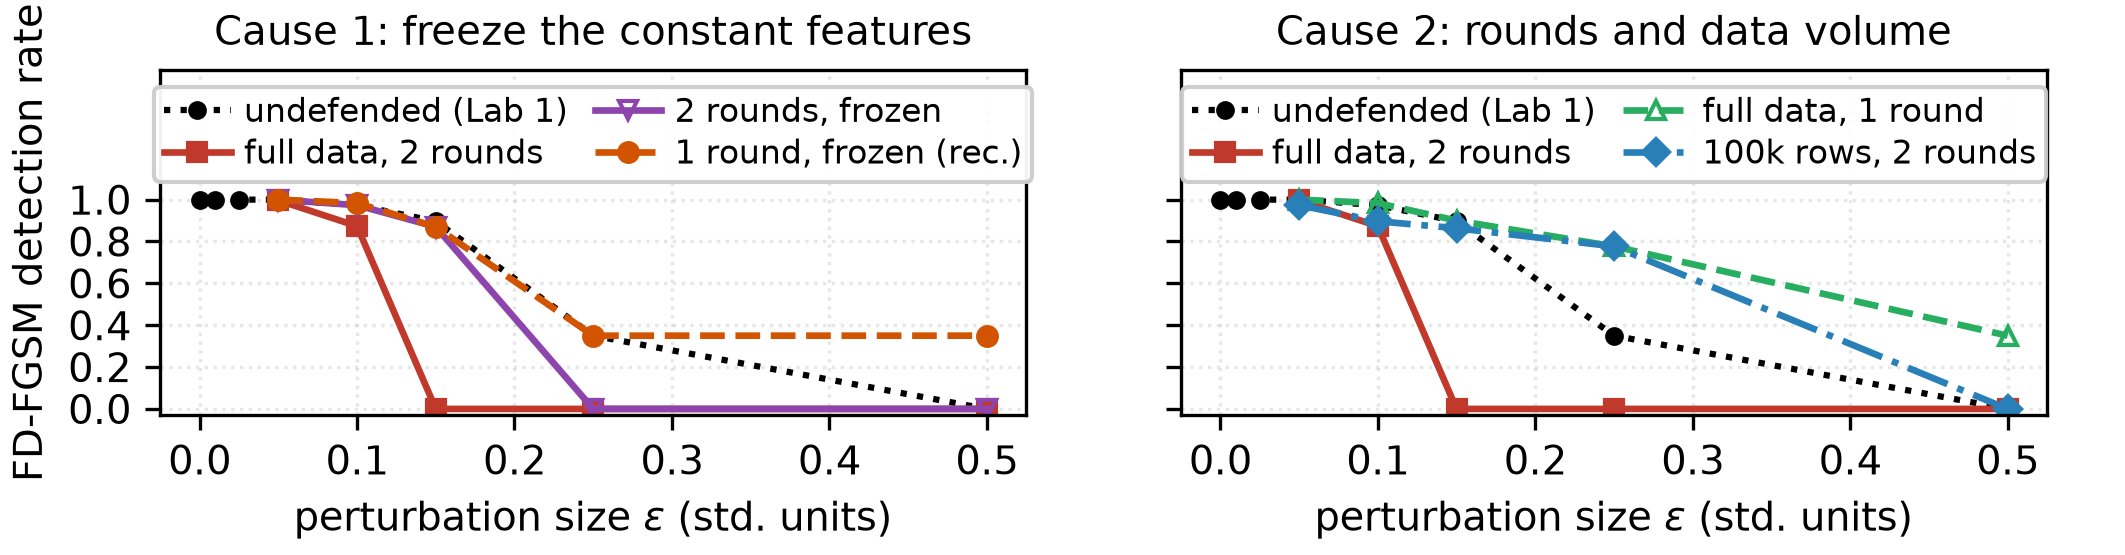
\includegraphics[width=0.62\textwidth]{task1c_ablation.png}
\caption{Ablation, FD-FGSM, same 300 flows. Left: freezing the ten constant features removes the collapse at $\vtheta=0.15$ (Cause 1). Right: at 0.25 the two-round full-data model sits at 0.000, while one round and the 100{,}000-row refit hold 0.777 (Cause 2).}\label{fig:ablation}
\end{figure}

\lead{Randomized smoothing and the certified radius.} Smoothing classifies many noisy copies of a flow and takes the majority vote. We used noise $\sigma=0.25$ standardized, $n=1{,}000$ samples, a statistical lower bound on the vote share (Clopper-Pearson), and 200 test flows on the two-round model. The certified radius is the size of change, measured as Euclidean length over all features together, that provably cannot flip the answer.
\begin{itemize}
\item \textbf{Radius.} The median certified radius is \textbf{R = 0.670} standardized units, with 0 abstentions and a median vote share of 1.000; the spread is small (p25 0.612, mean 0.617).
\item \textbf{Ceiling.} Even if all 1{,}000 noisy copies agree, we can only be sure of 99.63\% agreement. That caps the radius at $0.25\times2.6799=0.670$: the median is a ceiling set by $n$, not a measured margin.
\item \textbf{Not the attack we measured.} The certificate covers a round ball of change; our attack changes each feature separately, which reaches much further. In the two-round model's units the attack at $\vtheta=0.15$ reaches a Euclidean length of \textbf{2.87}, far beyond 0.670. The certificate therefore says nothing about the failure above.
\item \textbf{Detection under smoothing.} Smoothing did not raise detection. At $\vtheta=0.15$, PGD is detected on 0.297 of flows, and the adaptive attack (PGD averaged over 32 noise draws per step) on 0.300. The unsmoothed two-round model scores 0.350 against PGD. FD-FGSM is detected on 0.000 (0/300) at $\vtheta=0.15$, as unsmoothed.
\end{itemize}

\lead{What the defense costs.} Clean accuracy: nothing. Training: two CPU refits of 319.7\,s and 352.5\,s. Scoring one flow takes a median 0.12\,ms, the same as the Lab~1 model, so retraining adds no serving cost. Smoothing's 1{,}000 noisy copies took a median 0.43\,ms as one batch, on either model.

\lead{The one-round candidate.} Verdict: \S1. The candidate is the Lab~1 model adversarially trained for one round with the ten constant features frozen. It removes almost all of F8's extra risk (FD-FGSM at $\vtheta=0.15$ is slightly lower, see the ablation table), so F5's exposure (Medium) remains. Ship it only if it passes the evasion-curve release gate (Key terms), never a clean-accuracy gate.
\begin{itemize}
\item \textbf{Detection:} never lower than the Lab~1 model, except FD-FGSM at $\vtheta=0.15$ (261/300 flows detected against 269/300). It is higher at 0.10 (.983/.997 against .973, FD-FGSM/PGD-40) and, for PGD-40, at 0.25 (.777 against .350; FD-FGSM ties at .350). Clean accuracy is 1.000000.
\item \textbf{Membership-inference accuracy:} 0.5169 (95\% CI [0.5119, 0.5218]) against the blind control 0.5472, so no leak.
\item \textbf{Certified radius:} median 0.670, the same as the two-round model, with 0/200 abstentions.
\item \textbf{Detection under smoothing:} about the same as unsmoothed (FD-FGSM at $\vtheta=0.15$: 257/300 smoothed, 261/300 unsmoothed).
\end{itemize}
